\documentclass[UTF8]{ctexart}

\usepackage{geometry} 
\usepackage{setspace}
\usepackage{graphicx}

\geometry{left=30mm,right=30mm,top=25mm,bottom=25mm}
\setlength{\baselineskip}{30pt}

\title{\vspace{-1.5cm}第二部分需求文档\vspace{-2em}}

\date{}

\begin{document}
\maketitle
\section{综述}
本部分立足前端,对照饿了么网页版,制作与之高度相似的静态网页,其中包括首页、商家列表页面、商家信息页面、确认订单页面、在线支付页面、我的订单页面及登录与注册页面,并实现页面之间跳转、具体信息展示与隐藏等功能。

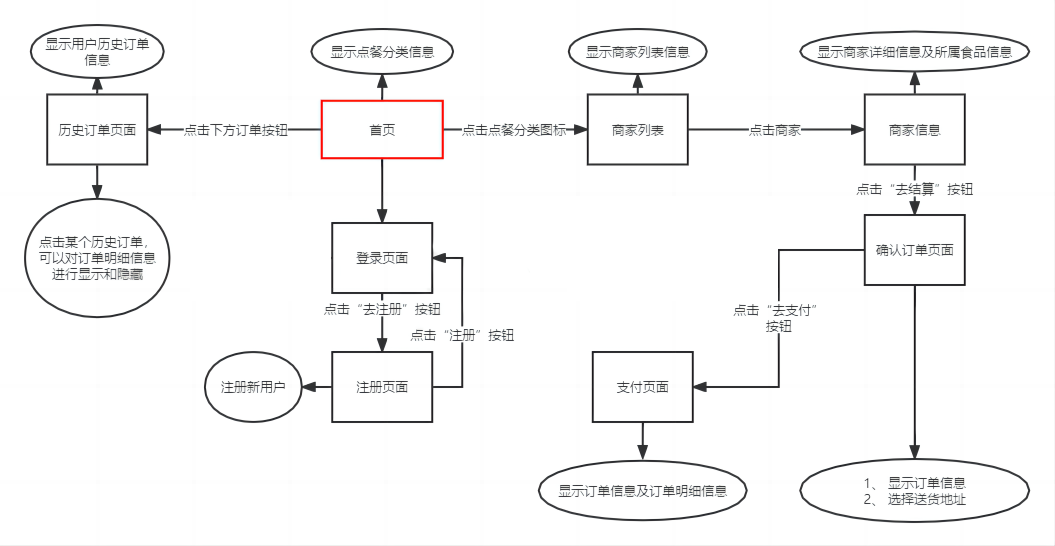
\includegraphics[width=1\textwidth]{第二部分}

\section{首页}
本部分展示商品分类及商家信息,并为用户提供搜索功能。其中搜索框固定在页面上方,底部菜单固定在页面下方。

首页包括以下动作:
\begin{itemize}
    \item \textbf{商品分类:}点击即可跳转商家列表页面,用于用户选择合适商家。
    \item \textbf{订单:}点击即可跳转我的订单页面,用于用户查找历史订单。
\end{itemize}

\section{商家列表页面}
本页面展示各商家信息及配送费等具体价格信息。

商家列表页面包括以下动作:
\begin{itemize}
    \item \textbf{商家列表中的各商家:}点击即可跳转商家信息页面,用于用户选购具体商品。
    \item \textbf{订单:}点击即可跳转我的订单页面,用于用户查找历史订单。
    \item \textbf{首页:}点击即可跳转首页。
\end{itemize}

\section{商家信息页面}
本页面展示某商家的所有商品信息及价格,并为用户提供增减商品功能。在用户选择商品完毕后可在底部菜单进行交互。若用户选择的商品价格达到配送标准,则显示去结算按钮;若未达到配送标准,则显示起送金额以提醒用户。

商家信息页面包括以下动作:
\begin{itemize}
    \item \textbf{去结算:}点击即可跳转确认订单界面,用于用户核对订单并做支付前确认。
    \item \textbf{订单:}点击即可跳转我的订单页面,用于用户查找历史订单。
    \item \textbf{首页:}点击即可跳转首页。
\end{itemize}

\section{确认订单页面}
本页面展示用户选择的收货地址、收货人信息、商家信息、订单详情与总价格。

确认订单页面包括以下动作:
\begin{itemize}
    \item \textbf{去支付:}点击即可跳转在线支付界面,用户可点击进入支付流程。
    \item \textbf{订单:}点击即可跳转我的订单页面,用于用户查找历史订单。
    \item \textbf{首页:}点击即可跳转首页。
\end{itemize}

\section{在线支付页面}
本页面展示简短的订单信息,包括商家信息及总价格,在订单信息下方为用户可选择的多种支付方式,用户可以选择其中一种支付方式进行支付。

在线支付页面包括以下动作:
\begin{itemize}
    \item \textbf{商家信息右侧倒三角图标:}点击可展示订单详细信息,再次点击可隐藏。
    \item \textbf{订单:}点击即可跳转我的订单页面,用于用户查找历史订单。
    \item \textbf{首页:}点击即可跳转首页。
\end{itemize}

\section{我的订单页面}
本页面展示用户的历史订单信息,未支付订单会显示未支付字样以提醒用户。

我的订单页面包括以下动作:
\begin{itemize}
    \item \textbf{商家信息右侧倒三角图标:}点击可展示订单详细信息,再次点击可隐藏。
    \item \textbf{首页:}点击即可跳转首页。
\end{itemize}

\section{登录页面}
本页面为用户登录页面,用户在手机号码和密码文本框中输入可进行登录。若用户未注册也可在此跳转注册页面。

登陆页面包括以下动作:
\begin{itemize}
    \item \textbf{手机号码/密码:}用户可在该文本框中输入手机号码或密码进行登录。
    \item \textbf{去注册:}点击即可跳转注册页面,用于新用户的注册。
    \item \textbf{订单:}点击即可跳转我的订单页面,用于用户查找历史订单。
    \item \textbf{首页:}点击即可跳转首页。
\end{itemize}

\section{注册页面}
本页面为用户注册页面,用户在手机号码和密码文本框中输入,进行确认密码并选择性别后可完成注册。

注册页面包括以下动作:
\begin{itemize}
    \item \textbf{手机号码/密码/确认密码:}用户可在该文本框中输入手机号码、密码并确认密码进行注册。
    \item \textbf{男/女:}用户可点击选择性别。
    \item \textbf{注册:}点击即可跳转登录页面,用于用户注册后进行登录。
    \item \textbf{订单:}点击即可跳转我的订单页面,用于用户查找历史订单。
    \item \textbf{首页:}点击即可跳转首页。
\end{itemize}

\end{document}
